\documentclass[a4paper,12pt]{article}
\usepackage{czech}
\usepackage[utf8]{inputenc}
\usepackage{a4wide}
\usepackage[dvipdfm]{graphicx}
\usepackage{graphics}
\usepackage{indentfirst}
\usepackage{fancyhdr}
\usepackage{setspace}
\usepackage{amsmath}
\usepackage{amssymb}
\usepackage{epsfig}

%%\usepackage{nopageno}
%%\usepackage{txfonts}
\usepackage[usenames]{color}

\begin{document}
\section{Úkol}
\noindent
\begin{enumerate}
    \item Změřte voltampérovou charakteristiku vakuové diody (EZ 81) pomocí zapisovače 4106
    \item Změřte voltampérovou charakteristiku Zenerovy diody (KZ 703) pomocí převodníku UDAQ-1408E.
    \item Pro Zenerovu diodu určete její dynamický vnitřní odpor v propustném směru při proudu 200 mA a v závěrném směru pro proud 400 mA.
    \item Určete odpovídající Zenerovo napětí $U_Z$.
    \item Zakreslete do V-A charakteristiky zatěžovací přímku pro napětí zdroje $U_1$ = -9 V a proud $I$ = 400 mA.
    \item Sestavte stabilizátor napětí a ověřte jeho funkci.
\end{enumerate}


\section{Teorie}
\subsection{Vakuová dioda}
Vakuová dioda je baňka, do které jsou zavedeny dvě elektrody. Uvnitř je vakuum, proto je pro průchod proudu dodat elektrony, které zpravidlá 
vznikají tepelnou emisí katody. Velikost emistího proudu $I$ je dán Richardonovým-Dushmanovým zákonem
\begin{eqnarray}
I=AST^2\exp{-w_0/kT},
\label{I1}
\end{eqnarray}
kde $A$ a $w_0$ jsou konstanty charakterizující emisní látku, $S$ plocha katody a $k$ Boltzmanova konstanta. Při nulovém napětí mezi elektrodami 
teče elektronkou proud řádově o velikost $10^{-5}$ až $10^{-4}$ A. To se dá ještě snížit záporným napětím na eletrodách, kdy se proud vytrácí asi 
při napětí $U=-1$V.

Velikost proudu v závislosti na nepětí je popsána přibližně rovnicí
\begin{eqnarray}
I=aU^{\frac{3}{2}},
\end{eqnarray}
kde $a$ je kontanta závislá na geometrickém uspořádání elektrod. Proud při zvyšování napětí roste až po hodnotu popsanou v rovnici \ref{I1}, kdy dosáhne 
nasicenosti a dále neroste.

\subsection{Zenerova dioda}
Zenerova dioda je speciální případ PN přechodu, který není zničen při proražení proudu v závěrném směru. Její VA charakteristika je na obrázku \ref{VAZ}.
\begin{figure}
\begin{center}
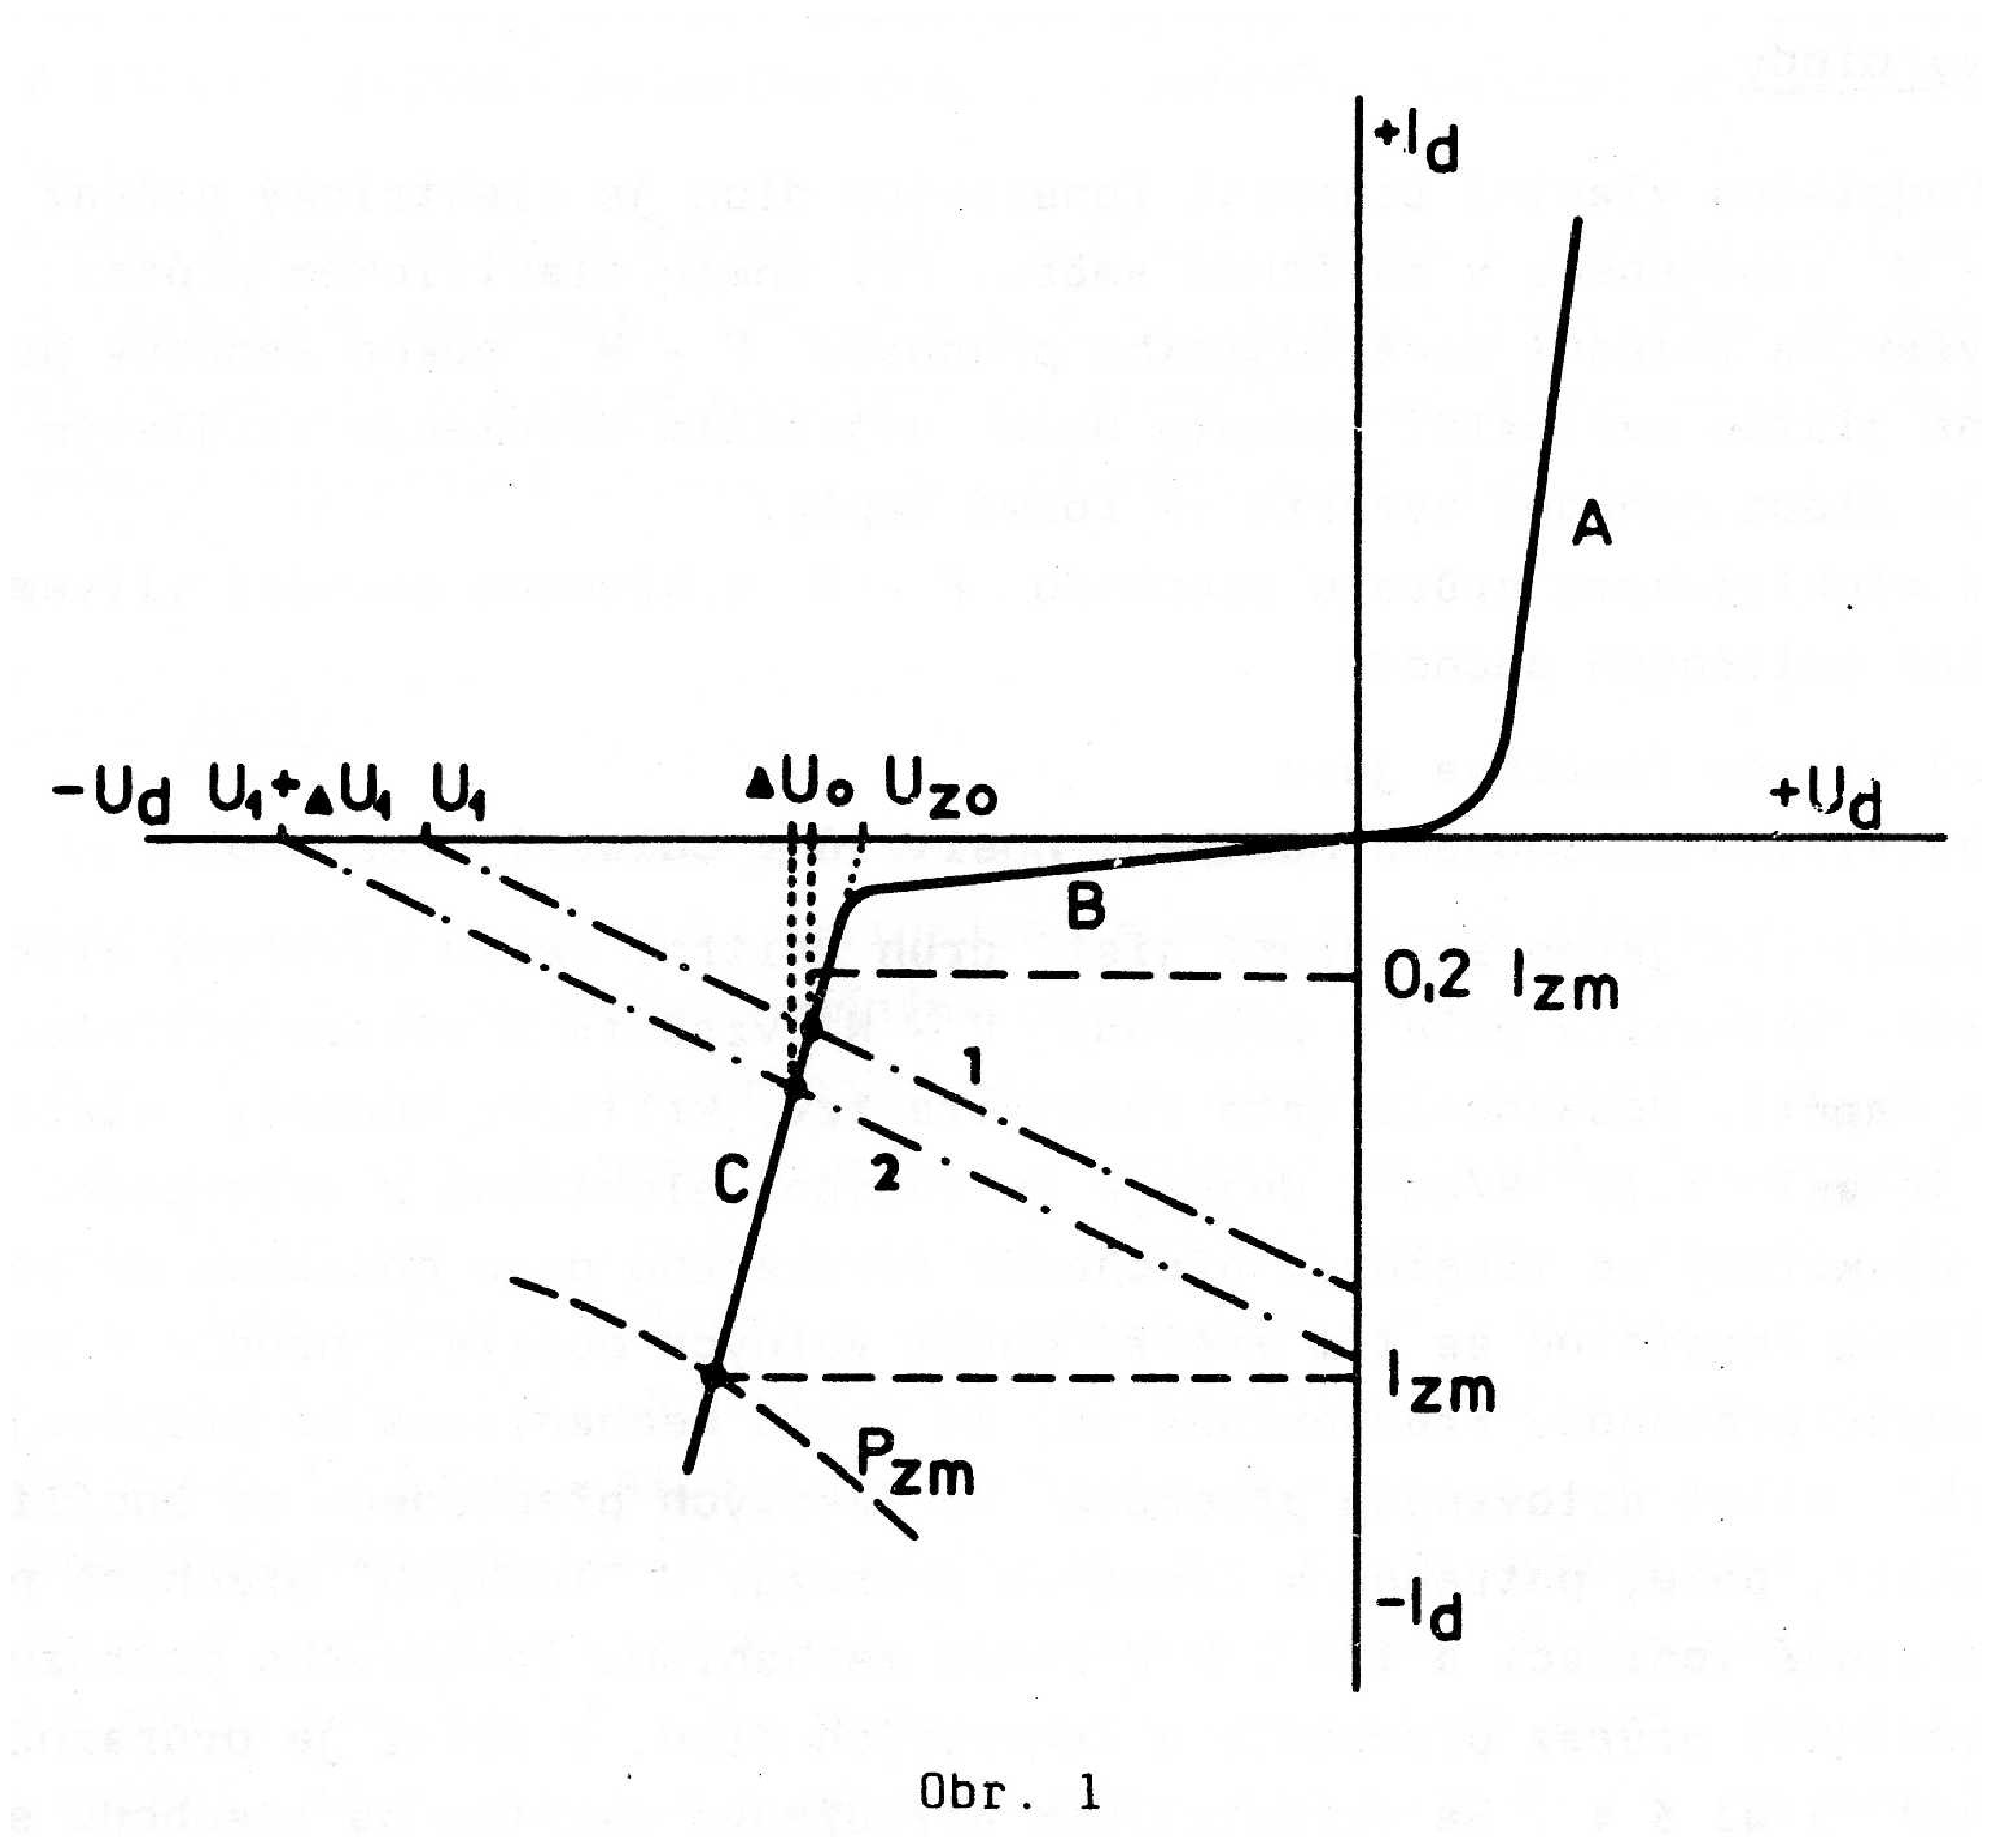
\includegraphics[scale=0.2]{VAZ.eps}
\caption{VA charakteristika Zenerovy diody}
\end{center}
\label{VAZ}
\end{figure}

Zenerova diona se dá použít jako stabilizátor napětí. Její účinost se popisuje stabilizačním činitelem, který je definován
\begin{eqnarray}
S=\frac{U_{out}}{U_{in}}\frac{\Delta U_{in}}{\Delta U_{out}}.
\end{eqnarray}

\subsection{Souřadnicový zapisovač}
Souřadnicový zaposovač je zařízení, které mění souřadnice pera v závislosti na napětí. V našem případě měříme na ose y napětí na odporu 5 $\Omega$, z čehož dle 
Ohmova zákonu snado dopočítáme odpovídající proud
\begin{eqnarray}
I=\frac{U}{R}.
\end{eqnarray}

\subsection{Chyby}
U zapisovače jsem bral jako chybu měřidla hodnotu odpovídající 0.5 mm, která ej závislá na zvoleném rozsahu a bude uvedena u každěho měření.

Dále jsem odečítal hodnoty z multimetrů MASTERTECH MY-65, které mají dle výrobce chybu na stejnosměreného napětí na rozsahu 20 V $\pm0.1\% \pm 3d$.

Dále jsem použil vztah pro chybu součinu a podílu veličin, kdy se relativní chyby sčítají.

\section{Měření}
\subsection{VA charakteristika vakuové diody}
Pomocí zapisovače jsem změřil VA charakteristiku vakuové diody. Výsledný graf je v příloze. Pro kladé hodnoty napětí (1) byl rozsah os
$y=50$mV/cm, $x=200$mV/cm. Pro závěrný směr (2) jsem změnil rozsah na $y=0.1$mV/cm, $x=200$mV/cm. Charakteristiku jsem také proměřil za 
pomoci počítače, který odečítal hodnoty z dvou multimetrů. Grafy jsou omět v příloze,

\subsection{VA charakteristika Zenerovy diody}
U VA charakteristiky Zenerovy diody (3) jsem již rozsah neměnil a pro celý graf byl rozsah os $y=500$mV/cm, $x=500$mV/cm.
Tuto charakteristiku jsem opět zpracoval za pomoci počítače a výsledný graf je v příloze.

\subsection{Dynamický vnitřní odpor Zenerovy diody}
Z grafu vytvořeným zapisovačem jsem určil dynamické vnitřní odpory pro proudy 200 mA v propustném směru a 400 mA v závěrném směru, a to tak, že jsem 
odečetl hodnoty v blízkosti hledané hodnoty a proložil je přímkou. Její převrácená hodnota směrnice je hledaný odpor. Odečtené hodnoty jsou v tabulkách \ref{TZ1} a \ref{TZ2}.
\begin{table}
$$
\begin{array}{|c|c|}
\hline
U/\mbox{V}& I/\mbox{mA} \\ \hline
0.80 \pm 0.03&  0.10 \pm 0.01 \\ \hline
0.85 \pm 0.03&  0.30 \pm 0.01 \\ \hline
0.90 \pm 0.03&  0.45 \pm 0.01 \\ \hline
0.95 \pm 0.03&  0.75 \pm 0.01 \\ \hline
\end{array}
$$
\caption{Charakteristiky Zenerovy diody pro propustný směr proudu.}
\label{TZ1}
\end{table}
\begin{table}
$$
\begin{array}{|c|c|}
\hline
U/\mbox{V}& I/\mbox{mA} \\ \hline
-7.05 \pm 0.03&  -0.40 \pm 0.01 \\ \hline
-7.10 \pm 0.03&  -0.50 \pm 0.01 \\ \hline
-7.15 \pm 0.03&  -0.70 \pm 0.01 \\ \hline
\end{array}
$$
\caption{Charakteristiky Zenerovy diody pro závěrný směr proudu.}
\label{TZ2}
\end{table}

Pro propustný směr vyšla hodnota dynamického odporu $R=(0.24\pm0.02)\Omega$, pro závěřný 
$R=(0.33\pm0.06)\Omega$.

\subsection{Pracovní bod a Zenerovo napětí}
Do grafu jsem dle zadání zanesl přímku odpovídající napětí -9 V a proudu 400 mA. Tak jsem získal 
dopovídající Zenerovo napětí, jehož hodnota je $U_z=(6.95\pm0.3)\mbox{V}$.

\subsection{Stabilizátor napětí}
Sestavil jsem usměrňovač napětí a proměřil jeho funkčnost. Výsledky jsou v tabulce \ref{TS} spolu 
s odpovídajícím stabilizačním koeficientem.
\begin{table}
$$
\begin{array}{|c|c|c|}
\hline
U_{in}/\mbox{V}&    U_{out}/\mbox{V}&   S \\ \hline
7.058 \pm 0.007&   6.942 \pm 0.007&  \\ \hline
7.580 \pm 0.008&   6.985 \pm 0.007& 11.19 \pm 0.04 \\ \hline
8.027 \pm 0.008&  7.009 \pm 0.007&  16.26 \pm 0.06 \\ \hline
8.559 \pm 0.009&   7.035 \pm 0.007& 16.81 \pm 0.06 \\ \hline
9.026 \pm 0.009&   7.060 \pm 0.007& 14.61 \pm 0.05 \\ \hline
9.521 \pm 0.010&  7.086 \pm 0.007&  14.16 \pm 0.05 \\ \hline
10.03 \pm 0.01&  7.117\pm 0.007&    11.61 \pm 0.04 \\ \hline
10.56 \pm 0.01& 7.145\pm 0.007&     12.95 \pm 0.04 \\ \hline
11.00 \pm 0.01& 7.169 \pm 0.007&    11.89 \pm 0.04 \\ \hline
11.52 \pm 0.01&  7.198 \pm 0.007&   11.14 \pm 0.04 \\ \hline
12.08 \pm 0.01& 7.229\pm 0.007&     10.90 \pm 0.04 \\ \hline
\end{array}
$$
\caption{Závislost výstupního napětí na vstupním pro stabilizační obvod}
\label{TS}
\end{table}

\section{Diskuze}
Měření na zapisovači bylo přesnější, než jsem očekával, a to díky velké škále rozsahů, který na něm byly k dispozici. 
Díky tomu je vzniklá chyba pouze v řádu procent. Menší problém vzikl volbou pera, které zaprvé v počátku zápisu vytvořilo 
znatelnou kaňku.To se však dalo také dobře využít pro jeho nalezení. Zadruhé pero vynechávalo při rychlejší změně výchylky, 
což se projevilo především u VA charakteristiky Zenerovy diody, kdy u malé změny napětí, které se volilo na zdroji došlo k 
velké změné proudu a zdroj neměl dostatečnou citlivost pro výkres celistvé křivky. Další drobná chyna byla zplsobena pozicováním 
papíru, který u grafu Zenerovy diody zřejmě nebyl vodorovně s osou y.

Měřící přístroje napojené na počítač se ukázaly být mnohem rychlejší a přesnější. Díky hustému vzorkování navíc klesá 
statistická chyba. Výstupní graf však podle mě neposkytuje dostatečně přesná data na zpracování a musel bych vyhodnocovat přímo 
naměřené hodnoty. Navíc je podle mě v makru tvořící graf špatně zadaná jednotka na ose y, protože pochybuji, že by Zenerova dioda snesla 
proud o velikosti 1 kA.

Zenerova dioda se ukázala jako dobrý stabilizátor. Krajní hodnoty, které jsem prověřoval bych bral s rezervou, protože byly velmi blízko 
Zenerovu napětí a proto není vidět jasná závislost $S$ na vstupním napětí.

\section{Závěr}
Změřil jsem VA charakteristiku vakuové diody za pomoci souřadnicového zapisovače a převodníku. \\
Změřil jsem VA charakteristiku Zenerovy diody za pomoci souřadnicového zapisovače a převodníku. \\
Určil jsem dynamický odpor Zenerovy diody pro proudy 200 mA resp. -400 mA
\begin{eqnarray}
R&=&(0.24\pm0.02)\Omega,\mbox{resp.} \\
R&=&(0.33\pm0.06)\Omega,
\end{eqnarray}
Určil jsem Zenerovo napětí pro pracovní bod dle zadání
\begin{eqnarray}
U_z=(6.95\pm0.3)\mbox{V}.
\end{eqnarray}
Ověřil jsem funkci stabilizátoru.

\begin{thebibliography}{5}
	\bibitem{text} \textbf{Studijní text na praktikum II} \\http://physics.mff.cuni.cz/vyuka/zfp/txt\_211.pdf (18. 11. 2011)
    \bibitem{chyba} \emph{J. Englich}: \textbf{Zpracování výsldků fyzikálních měření} \\ LS 1999/2000
\end{thebibliography}




\end{document}
